\section{Future Work}

\subsection{Enhancing the Current Approach}
While the current models, particularly the 
Neural Network and Random Forest, delivered comparable 
and promising results, there are several areas for 
improvement. For both models, further fine-tuning of 
hyperparameters could enhance performance. 
In the case of the Neural Network, exploring learning 
rate scheduling, advanced regularization techniques, 
and different architectures might improve generalization 
and reduce overfitting. Similarly, for the Random Forest, 
optimizing parameters such as the number of trees, depth, 
and split criteria could yield better results.

Additionally, more sophisticated methods for handling 
class imbalance, such as ADASYN or class-specific loss 
functions, could improve accuracy for underrepresented 
classes. Beyond model tuning, exploring alternative 
approaches for feature extraction from text data, 
such as word embeddings (e.g., Word2Vec or BERT), 
topic modeling, or more advanced natural language 
processing techniques, could provide richer 
representations of the data and further boost 
performance across all models.

\subsection{Regression Analysis on Wine Prices}
In addition to improving the existing classification 
models, future work could extend the analysis to a 
regression task focused on predicting wine prices. 
Implementing regression models to predict continuous 
variables, such as wine prices, would involve 
developing and training models specifically tailored 
for regression tasks, such as Linear Regression, 
Decision Trees for Regression, and Neural Networks
with regression output layers.

The inclusion of price prediction could offer valuable 
insights into the factors that influence wine pricing, 
beyond just classification of wine varieties. 
This would involve preprocessing data for regression, 
exploring feature engineering techniques, and 
evaluating model performance using appropriate 
regression metrics (e.g., Mean Absolute Error, Mean Squared Error). 
Combining these regression results with the 
current classification models could provide a 
more comprehensive understanding of wine reviews 
and their impact on pricing.

\begin{figure}[H]
    \centering
    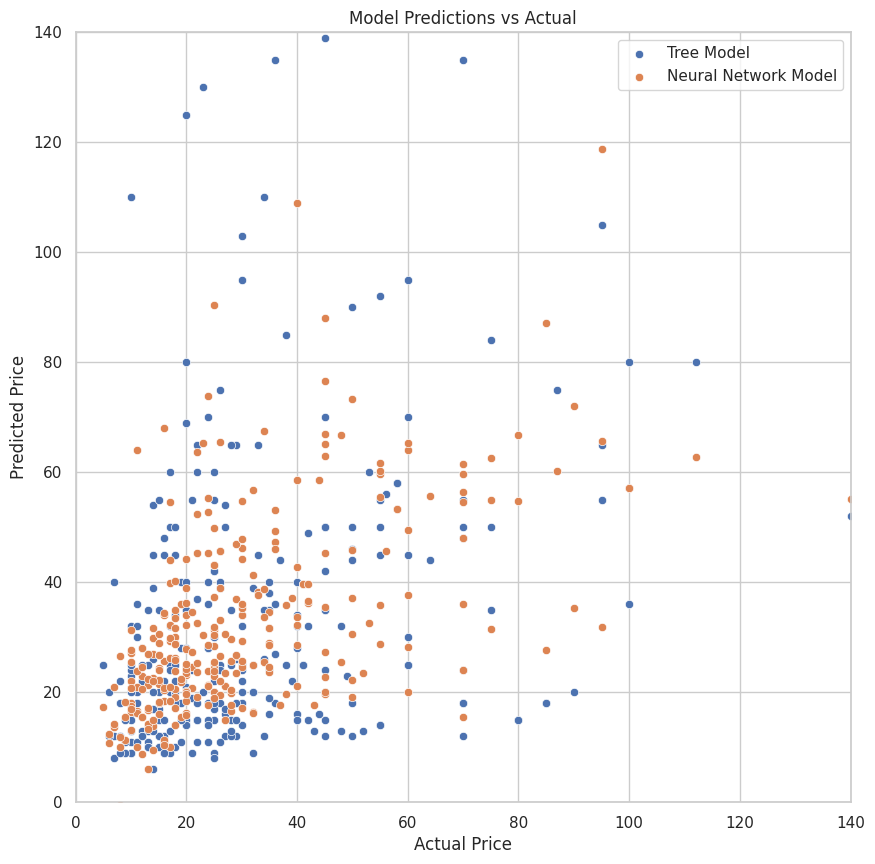
\includegraphics[width=0.99\columnwidth]{images/scatter_regressor_price.png}
    \caption{Predicted vs. Actual wine Prices}
    \label{fig:scatter_regressor_price}
\end{figure}